\subsubsection{\stid{6.02} LLNL ATDM: Flux}

\paragraph{Overview}

Flux~\cite{Ahn:2014:Flux,FluxSC18} is a next-generation resource
management and scheduling software framework under active development at
LLNL. This ECP project significantly augments the design and development
of this framework to address two specific technical challenges pertaining
to exascale computing.

\begin{enumerate}
\item Provide Flux as a portable user-level scheduling solution for complex
      exascale workflows

\item Provide capabilities for co-scheduling, high throughput, task
      coordination, and high portability.

\item Develop a resource model capable of portably representing job
      requirements of exascale systems.

\item Provide Flux as the system resource manager and scheduler for exascale
      systems.
\end{enumerate}

Major efforts include developing and deploying additional capabilities
such as management and scheduling of a diverse set of emerging workflows
as well as a diverse set of exascale resources (e.g., power and burst
buffers). The project strives to do this through co-design efforts with
major workflow management software development teams within ASC (i.e.,
LLNL’s UQPipeline), ECP/ATDM programs, and exascale computing hardware
vendors themselves. Because Flux’s design allows it to be used as a
user-space scheduling tool, it is suitable for co-development with other
workflow systems that require advanced scheduling capabilities. As a
system tool, it is a potential replacement for resource managers such as
SLURM, providing more advanced scheduling capabilities with full
awareness of resources beyond just nodes and CPUs (e.g., filesystems,
power, accelerators).


\paragraph{Key Challenges}

Exascale resource management is particularly complex as it requires us to
manage both the complexity of workloads (workflows, jobs, and services)
as well as the increasing complexity of exascale machines themselves.
Exascale systems may have diverse node types with CPUs, GPUs, burst
buffers, and other independently allocatable hardware resources. Jobs
must be mapped to these systems generically -- one application must be
able to run protably {\it and} with high performance or throughput on
{\it any} exascale machine.  Flux aims to save application developers the
pain of configuring and setting up their applciations and workflows
across multiple machine, and to enable massive ensembles and workflows to
run scalably on these machines.

\paragraph{Solution Strategy}

Flux implements {\it hierarchical} scheduling.  Ultimately, it will be
usable either as a full system resource manager, {\it or} as a scheduler
for a single workflow {\it within} another allocation, {\it or} as both.
Flux allows application-level workloads to choose their own scheduleing
policies and to specify concisely and portably the types of resources
they need to run on a range of machines.  Unlike prior approaches like
SLURM, which use a on-size-fits-all scheduling and job management
appoach, Flux allows the system to set global allocation policies, but
users can instnatiate their own schedulers and request specific resources
within an allocation.  With Flux, users have the control over policy and
scalability that was previously only tunable at the system level.


\paragraph{Recent Progress}

\begin{figure}[tb]
\centering
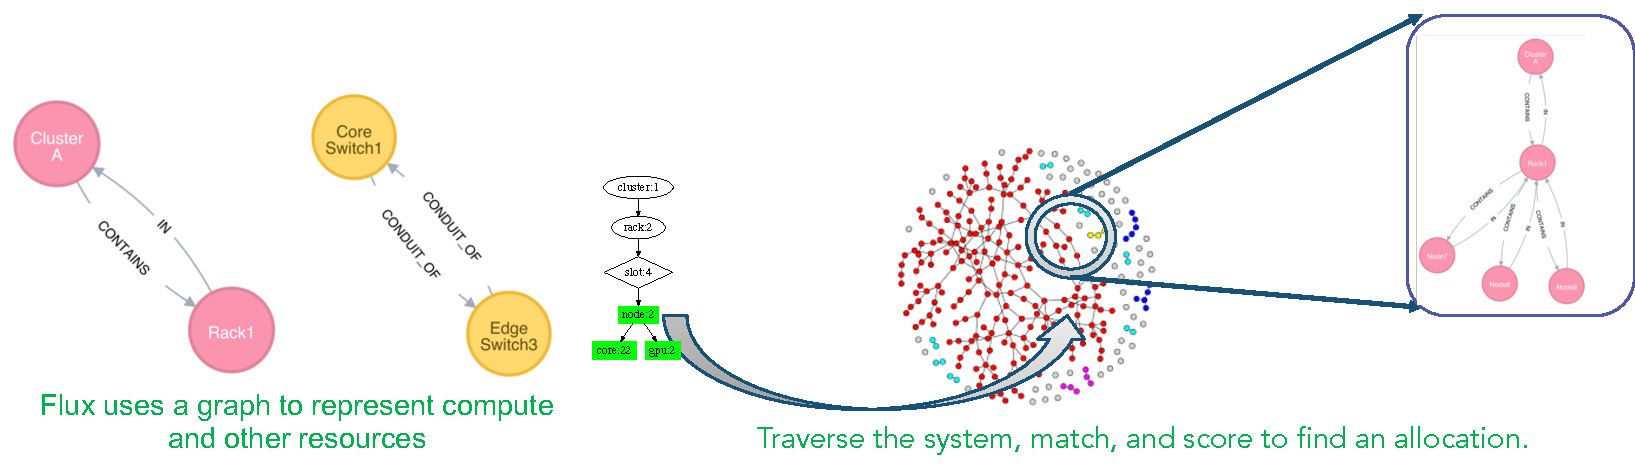
\includegraphics[width=\textwidth]{projects/2.3.6-NNSA/2.3.6.02-LLNL-ATDM/flux-resource-model.pdf}
\end{figure}

\begin{itemize}

\item Extended graph-based resource model to support multi-user systems. This
      enables Flux to be used as a full-system resource manager, with security
      and isolation among usres

\item Demonstrated end-to-end capability of DYAD data movement subsystem for LBANN.

\item Completed definition of workflow exception/error handling model.

\item Enabled two major scientific workflows to complete their calculations on
      LLNL’s Sierra pre-exascale systems.

\item Released flux-core 0.11 and flux-sched 0.7 that contain all of the
      functionalities used by these workflows.

\item Started to broaden outreach and collaboration across ECP (e.g., scheduler
      integration working group), DOE complexes (e.g., ORNL, SNL and LANL),
      universities (e.g., UTK) and vendors (e.g., IBM T.J. Watson).

\end{itemize}


\paragraph{Next Steps}

\begin{itemize}
\item Deeper integration wtih Cancer Moonshot Pilot2 code, and LLNL ML initiative.
\item Deeper LLNL UQ Pipeline integration.
\item Testing of LLNL MARBL code with Flux on the SNL Astra system.
\end{itemize}
.
